%
% File: chap01.tex
% Author: Zeller Quentin
% Description: Introduction
%
%\let\textcircled=\pgftextcircled
\chapter{OpenCV}
\label{chap:OpenCV}

\initial{O}penCV est une librairie multiplate-forme et open source pr�vue pour le machine learning ainsi que pour le traitement d'image (computer vision). Du fait de sa licence BSD, cette librairie est constamment am�lior�e par le march�, ce qui en fait une des librairies leader dans ce domaine. En plus d'�tre disponible sur la quasi totalit� des syst�me d'exploitation du march� elle �galement disponible dans multiple langage que sont : C++, C, Python, Java and MATLAB � ce jour. Nous utiliserons ici la librairie pour Python qui est un langage certes moins optimis� que certains de ses concurrents mais qui � l'instar de Mathlab permet de se concentrer sur le c?ur du sujet. Il dispose en outre d'une bonne communaut� et d'un bon support.



%=======
\section{Fonctionnement g�n�ral}
\label{sec:sec32a}
\section{Environnement de d�veloppement}
\label{sec:sec03b}
du texte

\subsection{Opera TV Emulator}
\label{subsec:subsec03b}

\begin{figure}[h]
	\centering
	\frame{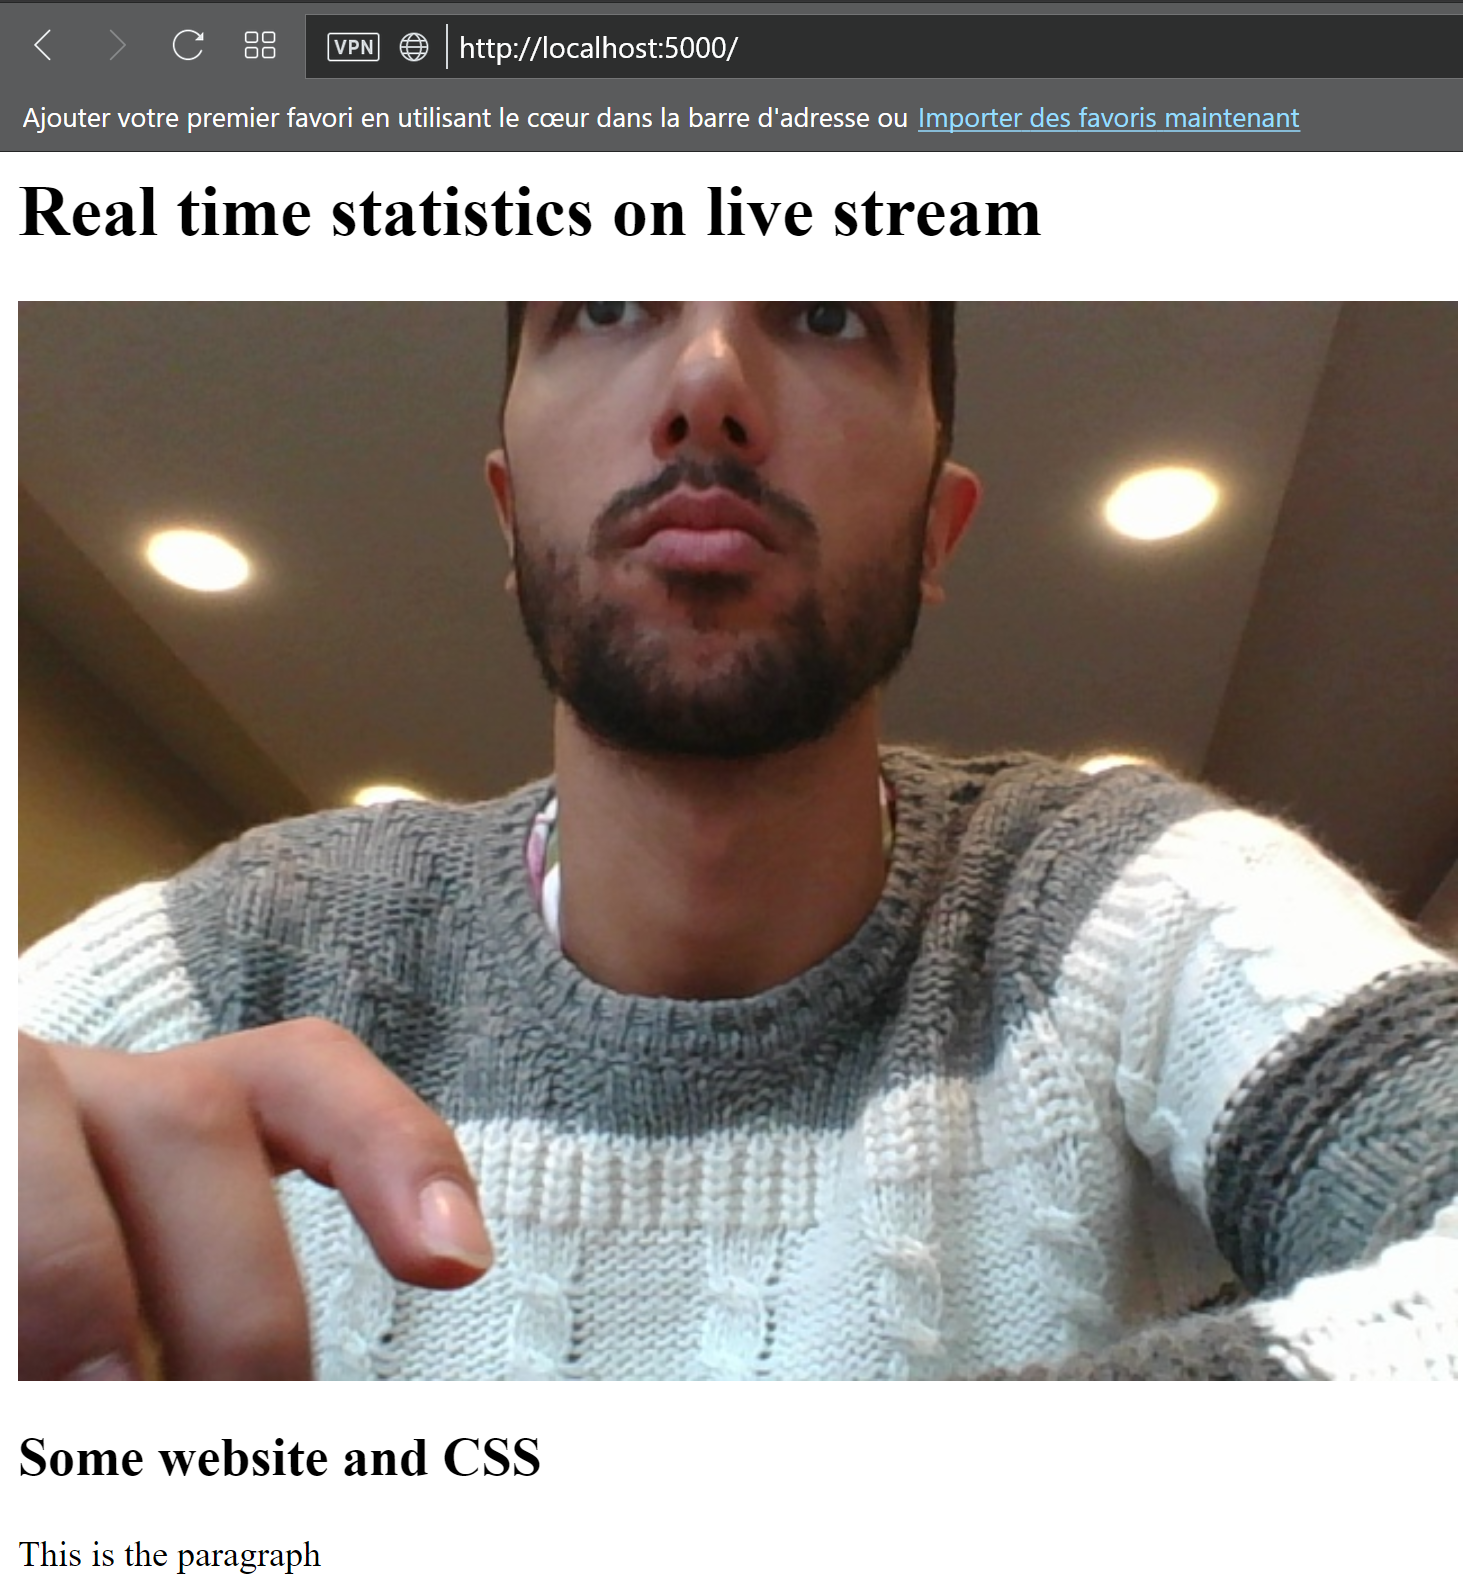
\includegraphics[width=0.8\linewidth]{fig01/website}}
	\mycaption[The easy Flask website MJPEG.]{Streaming HTTP avec librairie python Flask}
	\label{fig:flask}
	
\end{figure}
du texte
\begin{figure}[h]
	\centering
	\frame{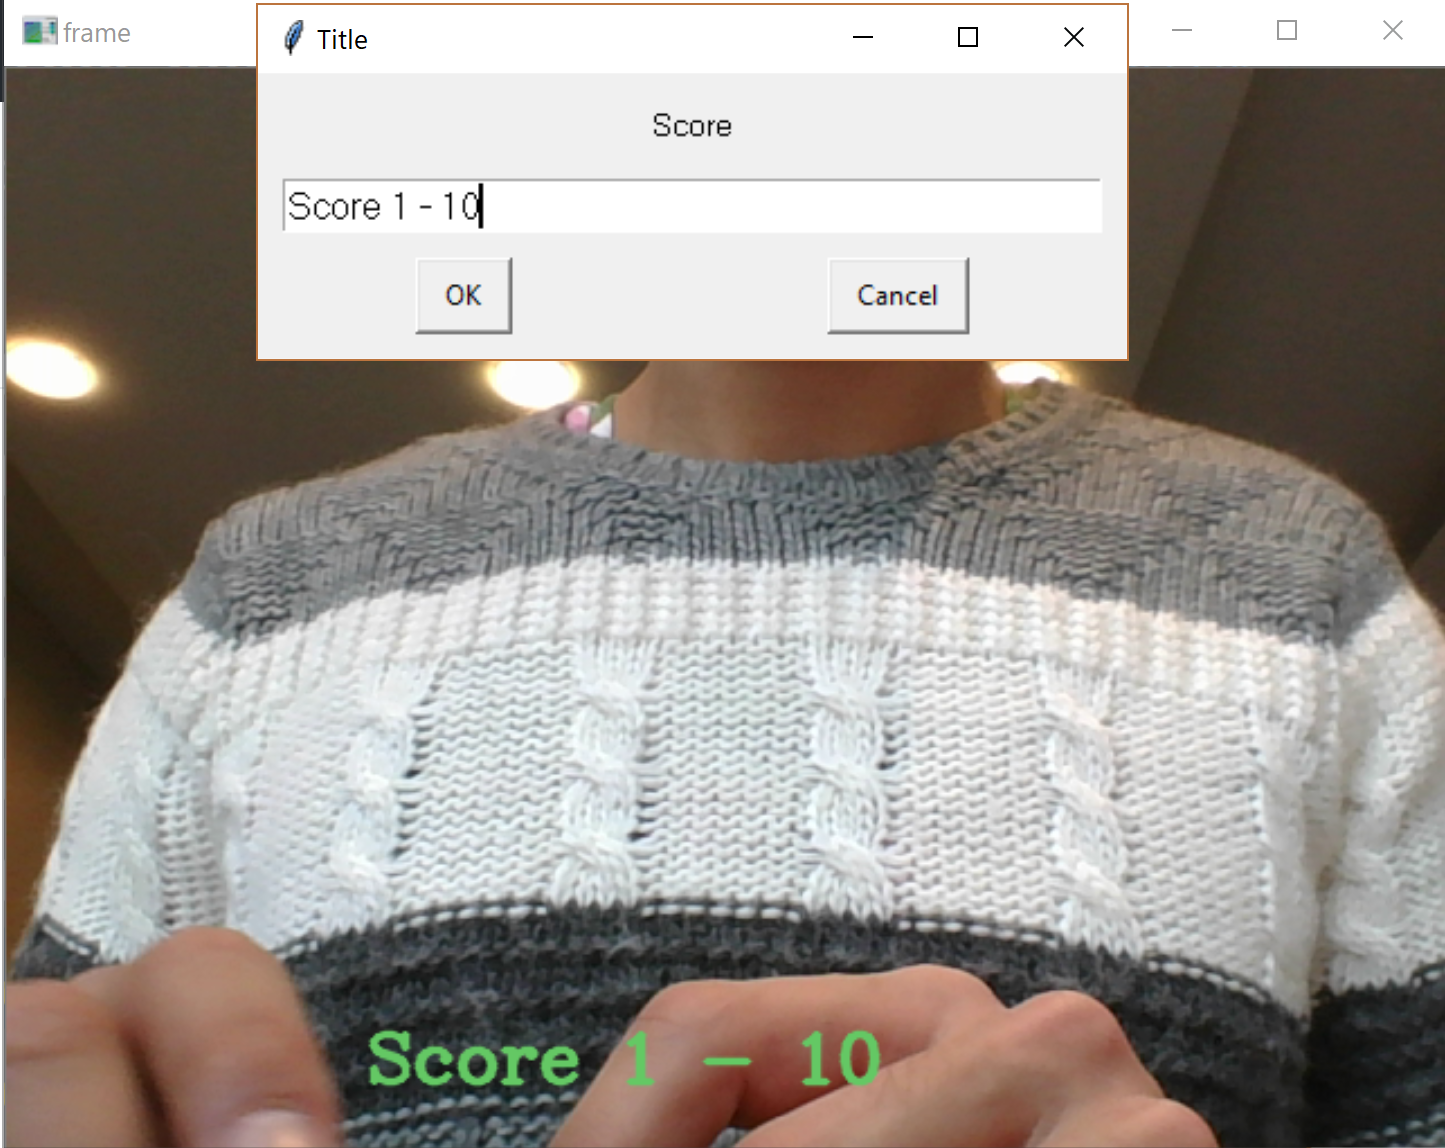
\includegraphics[width=0.8\linewidth]{fig01/example_application}}
	\mycaption[Burn text on live stream, display on GUI]{Int�gration texte dans vid�o live, affichage GUI bureau}
	\label{fig:live_text_integration}
	
\end{figure}
du texte
\begin{figure}[h]
	\centering
	\frame{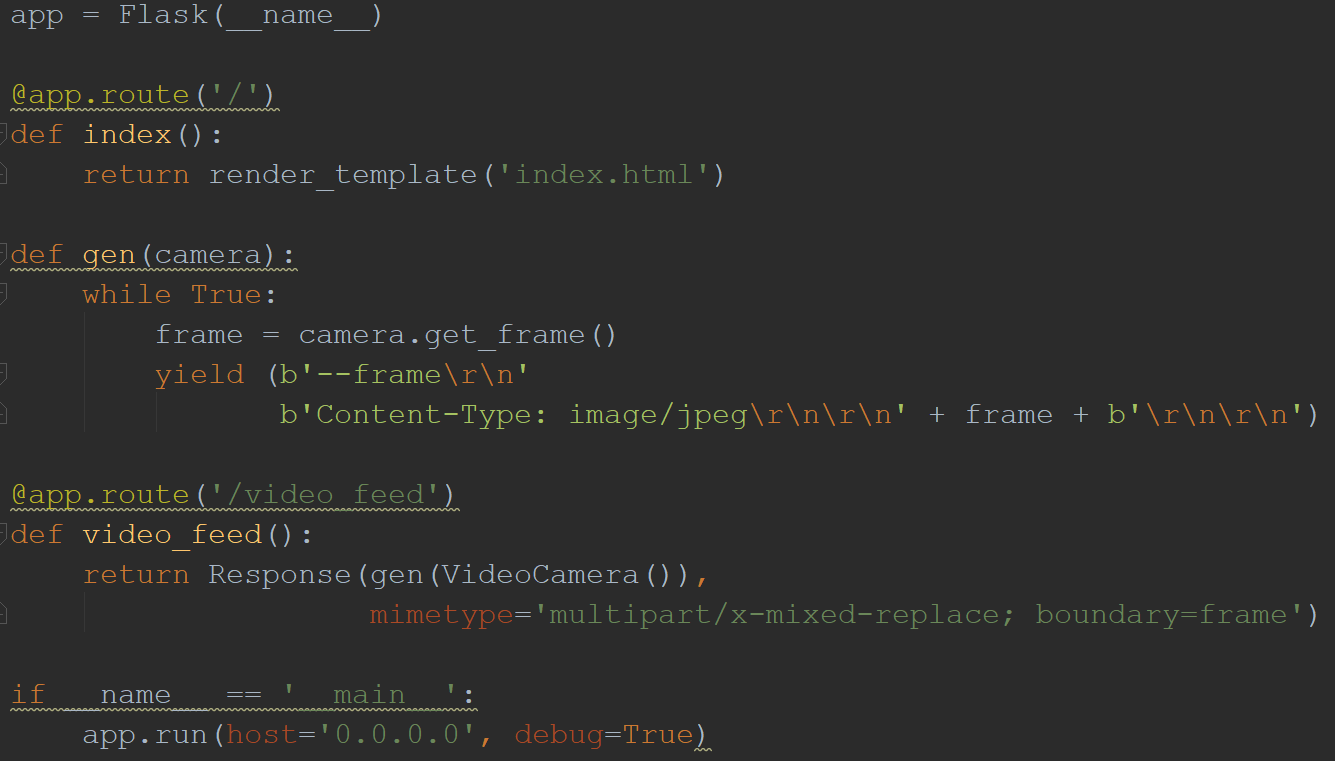
\includegraphics[width=1\linewidth]{fig01/flask_simple}}
	\mycaption[The easy Flask website MJPEG. (code)]{Code pour streaming HTTP avec librairie python Flask}
	\label{fig:flask_code}
	
\end{figure}


\section{Environnement de production}
\label{sec:sec03c}
\subsection{The Opera hybrid TV option}
\label{subsec:subsec03c}


%=========================================================